\usetikzlibrary{fit,shapes.arrows}
\newcommand{\cmark}{\ding{51}}%
\newcommand{\xmark}{\ding{55}}%
\begin{figure}
\centering
\resizebox{\columnwidth}{!}{%
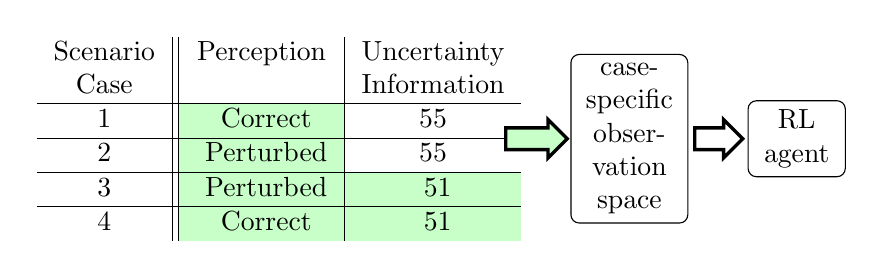
\begin{tikzpicture}
    \definecolor{hellgruen}{RGB}{200,255,200}


    \node (tabelle) {
        \begin{tabular}{c||c|c}
            Scenario & Perception & Uncertainty \\ 
            Case &  & Information \\ \hline
            1 & \cellcolor{hellgruen} Correct & \xmark \\ \hline
            2 & \cellcolor{hellgruen} Perturbed & \xmark \\ \hline
            3 & \cellcolor{hellgruen} Perturbed & \cellcolor{hellgruen} \cmark \\ \hline
            4 & \cellcolor{hellgruen} Correct & \cellcolor{hellgruen} \cmark \\
        \end{tabular}
    };

    \coordinate (a) at (2.9,0);
    \coordinate (b) at (3.5,0);
    \coordinate (c) at (3.2,0);
    \coordinate (d) at (5.45,0);

    \coordinate (e) at (5.3,0);
    \coordinate (f) at (5.73,0);
    
    \node[single arrow, draw=black, very thick, fill=hellgruen,
      minimum width = 10pt, single arrow head extend=3pt,
      inner xsep=0pt,
      fit=(a) (b)] {};

    \node[single arrow, draw=black, very thick, fill=white,
      minimum width = 10pt, single arrow head extend=3pt,
      inner xsep=0pt,
      fit=(e) (f)] {};

    \node[
        draw=black,
        rounded corners=3pt,
        fill=white,
        align=center,
        anchor=west,
        xshift=0.5cm,
        text width=1.25cm
    ] at (c) {case-specific observation space};

    \node[
        draw=black,
        rounded corners=3pt,
        fill=white,
        align=center,
        anchor=west,
        xshift=0.5cm,
        text width=1.0cm
    ] at (d) {RL agent};

\end{tikzpicture}
}
\caption{We consider four scenarios differing in perturbation of the observation space as well as the availability of the uncertainty information. Green color indicates the scenario-dependent components of the observation space.}
\label{fig:expsetup}
\end{figure}